\documentclass[11pt]{article}
\usepackage{setspace}
\setstretch{1}
\usepackage{amsmath,amssymb, amsthm}
\usepackage{graphicx}
\usepackage{bm}
\usepackage[hang, flushmargin]{footmisc}
\usepackage[colorlinks=true]{hyperref}
\usepackage[nameinlink]{cleveref}
\usepackage{footnotebackref}
\usepackage{url}
\usepackage{listings}
\usepackage[most]{tcolorbox}
\usepackage{inconsolata}
\usepackage[papersize={8.5in,11in}, margin=1in]{geometry}
\usepackage{float}
\usepackage{caption}
\usepackage{esint}
\usepackage{url}
\usepackage{enumitem}
\usepackage{subfig}
\usepackage{wasysym}
\newcommand{\ilc}{\texttt}
\usepackage{etoolbox}
\usepackage{algorithm}
\usepackage{changepage}
% \usepackage{algorithmic}
\usepackage[noend]{algpseudocode}
\usepackage{tikz}
\usetikzlibrary{matrix,positioning,arrows.meta,arrows}
\patchcmd{\thebibliography}{\section*{\refname}}{}{}{}
% \PassOptionsToPackage{hyphens}{url}\usepackage{hyperref}

\providecommand{\myceil}[1]{\left \lceil #1 \right \rceil }
\providecommand{\myfloor}[1]{\left \lfloor #1 \right \rfloor }


\begin{document}



\title{\textbf{CSDS 455: Homework 27}}


\author{Shaochen (Henry) ZHONG, \ilc{sxz517}}
\date{Due and submitted on 12/02/2020 \\ Fall 2020, Dr. Connamacher}
\maketitle



\section*{Problem 1}

\textit{Read sections 5 and 6 of the paper, and in your own words explain why they are able to bound the norm of the matrix by looking at the size of a separator set.}\newline

Known the tracing power $tr((MM^T)^q) \geq ||M^{2q}||$ (due to some supposely well-know linear stuffs that I don't know). We are interesting in finding the non-zero expected value of this $tr((MM^T)^q)$. By doing the constraint graph, we discovered that if a constraint graph $c$ has edge that not appeared in even time, it has a non-zero expected value. Like the orange and yellow edges in the following graph.


\begin{figure}[H]
    \centering
    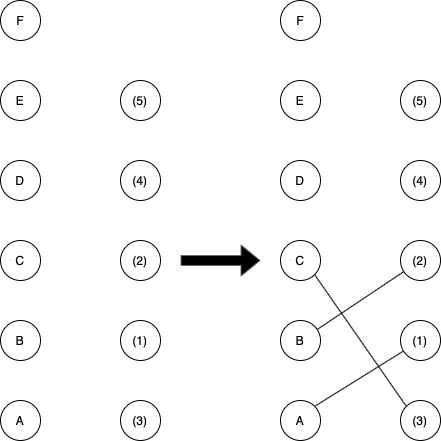
\includegraphics[width=0.4\linewidth]{{fig/fig_1.png}}
\end{figure}

Thus, wheather or not a constraint graph $c$ may have non-zero expected value for its tracing power will related to the distinct indicies it has. Let $S$ being the minimum vertex cut between shapes $U$ and $V$ in $H$. For distinct indicies, we know that the upper bound will be $|V(H)|q$ as every index can at most appear $q$ times. Each $p \in S$ will lower this bound by $q - 1$ (why?).

Then with \textsc{Menger's Theorem} we know that the maximum size of $S$ is dependend on the smaller of $U$ or $V$. WLOG we assume it is $|V|$ then we may update the bound to be $|V(H)|q - S(q - 1)$. As it bounds the tracing power, it therefore bounds the norm $||M^{2q}||$ due to the shown inequality.\newline


\noindent\textit{I have refered A LOT (if not straightly taken) from the Lecture 12 slide of \url{https://canvas.uchicago.edu/courses/17604}.}\newline



% Credit to Peter Grill on https://tex.stackexchange.com/questions/58901/something-between-frownie-and-smiley/59125
\newcommand{\Simley}[1]{%
\begin{tikzpicture}[scale=0.11]
    \newcommand*{\SmileyRadius}{3.0}%
    \draw [fill=brown!10] (0,0) circle (\SmileyRadius)% outside circle
        %node [yshift=-0.22*\SmileyRadius cm] {\tiny #1}% uncomment this to see the smile factor
        ;

    \pgfmathsetmacro{\eyeX}{0.5*\SmileyRadius*cos(30)}
    \pgfmathsetmacro{\eyeY}{0.5*\SmileyRadius*sin(30)}
    \draw [fill=cyan,draw=none] (\eyeX,\eyeY) circle (0.15cm);
    \draw [fill=cyan,draw=none] (-\eyeX,\eyeY) circle (0.15cm);

    \pgfmathsetmacro{\xScale}{2*\eyeX/180}
    \pgfmathsetmacro{\yScale}{1.0*\eyeY}
    \draw[color=red, domain=-\eyeX:\eyeX]
        plot ({\x},{
            -0.1+#1*0.15 % shift the smiley as smile decreases
            -#1*1.75*\yScale*(sin((\x+\eyeX)/\xScale))-\eyeY});
\end{tikzpicture}%
}%


ALL DONE \ \ \Simley{0} \Simley{0.1} \Simley{0.2} \Simley{0.3} \Simley{0.4} \Simley{0.5} \Simley{0.6} \Simley{0.7} \Simley{0.9} \Simley{0.9} \Simley{1} \ \ THANK YOU !!!!!!!!!!!!!!!!!!!!



\end{document}